% The authority figure: what each parameter can do to the peak-WSE error.
%
% Form: a line chart -- the data's job is change over a continuous parameter,
% and both series share BOTH axes honestly. x is a multiplicative factor on the
% parameter (alpha = n/n_prior for roughness, a = scale on the initial state),
% y is the same peak-WSE MAE in metres over the same 46 marks. That shared
% meaning is what makes one axis correct here; a dual-axis version would be
% meaningless.
%
% Both curves pass through the same point at 1.0 (the uncalibrated model), so
% the reader's eye lands on a shared anchor and the slopes do the arguing.
%
% Colour: categorical slots 1 and 2 of the validated palette (blue #2a78d6,
% orange #eb6834; adjacent-pair CVD dE 24.7 protan, 33.6 normal -- all six
% checks pass). Identity is never carried by colour alone: each series also has
% a distinct marker and dash pattern, so the figure survives greyscale printing.
%
% NB the axis spans 0.25-1.25 because the ROUGHNESS scan runs down to 0.30 --
% an earlier draft set xmin at 0.55 with clip=false and silently drew that
% curve outside the axis box.
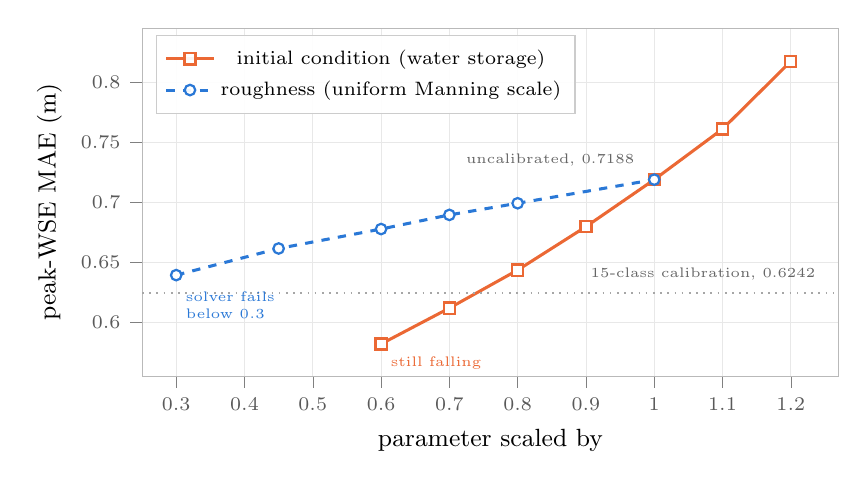
\begin{tikzpicture}
\begin{axis}[
  width=0.86\linewidth, height=6.0cm,
  xlabel={parameter scaled by},
  ylabel={peak-WSE MAE (m)},
  xmin=0.25, xmax=1.27,
  ymin=0.555, ymax=0.845,
  xtick={0.3,0.4,0.5,0.6,0.7,0.8,0.9,1.0,1.1,1.2},
  xticklabel style={/pgf/number format/fixed, /pgf/number format/precision=1},
  ytick={0.60,0.65,0.70,0.75,0.80},
  yticklabel style={/pgf/number format/fixed, /pgf/number format/precision=2},
  tick align=outside, tick pos=left,
  axis line style={gray!55},
  tick label style={font=\scriptsize, color=black!65},
  label style={font=\small},
  grid=major, grid style={gray!18, line width=0.3pt},
  legend style={font=\scriptsize, at={(0.02,0.98)}, anchor=north west,
                draw=gray!40, fill=white, fill opacity=0.93, text opacity=1,
                row sep=0.5pt, inner sep=3pt},
]

% --- initial condition: a scale on antecedent water storage (velocities fixed)
\addplot[color={rgb,255:red,235;green,104;blue,52}, line width=1.1pt,
         mark=square*, mark size=2.0pt, mark options={fill=white, line width=0.8pt}]
  coordinates {(0.6,0.5818) (0.7,0.6117) (0.8,0.6434) (0.9,0.6796)
               (1.0,0.7188) (1.1,0.7610) (1.2,0.8174)};
\addlegendentry{initial condition (water storage)}

% --- roughness: a uniform scale on the NLCD Manning field
\addplot[color={rgb,255:red,42;green,120;blue,214}, line width=1.1pt,
         dashed, mark=*, mark size=1.9pt,
         mark options={solid, fill=white, line width=0.8pt}]
  coordinates {(0.30,0.6392) (0.45,0.6614) (0.60,0.6776) (0.70,0.6894)
               (0.80,0.6991) (1.00,0.7188)};
\addlegendentry{roughness (uniform Manning scale)}

% --- the calibrated field: off both curves, since it redistributes
\addplot[gray!70, line width=0.6pt, dotted, forget plot]
  coordinates {(0.25,0.6242) (1.27,0.6242)};
\node[font=\tiny, color=black!60, anchor=south east]
  at (axis cs:1.25,0.6265) {15-class calibration, 0.6242};

% --- the shared anchor
\node[font=\tiny, color=black!60, anchor=south east]
  at (axis cs:0.985,0.7215) {uncalibrated, 0.7188};

% --- why each curve stops where it does
\node[font=\tiny, color={rgb,255:red,42;green,120;blue,214},
      anchor=north west, align=left]
  at (axis cs:0.30,0.6330) {solver fails\\below $0.3$};
\node[font=\tiny, color={rgb,255:red,235;green,104;blue,52},
      anchor=north west, align=left]
  at (axis cs:0.60,0.5790) {still falling};
\end{axis}
\end{tikzpicture}
